\documentclass[11pt]{article}

% "preprint" gives the non-anonymous version with page numbers (for arXiv);
% use "review" for an anonymized submission and "final" for camera-ready.
\usepackage[preprint]{acl}

\usepackage{times}
\usepackage{latexsym}
\usepackage[T1]{fontenc}
\usepackage[utf8]{inputenc}
\usepackage{microtype}
\usepackage{graphicx}
\usepackage{booktabs}
\usepackage{enumitem}
\usepackage{amsmath}
\usepackage{url}

\newcommand{\accZeroFin}{0.42}
\newcommand{\accFullFin}{0.18}
\newcommand{\ovZeroFin}{0.77}
\newcommand{\ovFullFin}{0.77}
\newcommand{\nliZeroFin}{0.62}
\newcommand{\nliFullFin}{0.59}
\newcommand{\vscZeroFin}{0.77}
\newcommand{\vscFullFin}{0.52}
\newcommand{\nFinCorrupt}{400}
\newcommand{\aucFinoverlap}{0.53}
\newcommand{\aucFinoverlapci}{[0.50, 0.56]}
\newcommand{\aucFinnli}{0.53}
\newcommand{\aucFinnlici}{[0.51, 0.56]}
\newcommand{\aucFinlexical}{0.52}
\newcommand{\aucFinlexicalci}{[0.50, 0.54]}
\newcommand{\aucFinnohalluc}{0.51}
\newcommand{\aucFinnohallucci}{[0.49, 0.52]}
\newcommand{\aucFinconf}{0.54}
\newcommand{\aucFinconfci}{[0.52, 0.55]}
\newcommand{\aucFincorrect}{0.65}
\newcommand{\aucFincorrectci}{[0.63, 0.67]}
\newcommand{\aucFinvsclean}{0.92}
\newcommand{\aucFinvscleanci}{[0.90, 0.94]}
\newcommand{\nFinErr}{982}
\newcommand{\errFinoverlap}{0.47}
\newcommand{\errFinnli}{0.55}
\newcommand{\errFinlexical}{0.53}
\newcommand{\errFinnohalluc}{0.51}
\newcommand{\errFinconf}{0.54}
\newcommand{\nFinRet}{800}
\newcommand{\missFin}{16}
\newcommand{\retFinoverlap}{0.49}
\newcommand{\retFinnli}{0.57}
\newcommand{\retFinlexical}{0.48}
\newcommand{\retFinnohalluc}{0.51}
\newcommand{\retFinconf}{0.53}
\newcommand{\retFincorrect}{0.66}
\newcommand{\accZeroTat}{0.53}
\newcommand{\accFullTat}{0.06}
\newcommand{\ovZeroTat}{0.78}
\newcommand{\ovFullTat}{0.77}
\newcommand{\nliZeroTat}{0.33}
\newcommand{\nliFullTat}{0.31}
\newcommand{\vscZeroTat}{0.78}
\newcommand{\vscFullTat}{0.58}
\newcommand{\nTatCorrupt}{300}
\newcommand{\aucTatoverlap}{0.53}
\newcommand{\aucTatoverlapci}{[0.50, 0.56]}
\newcommand{\aucTatnli}{0.50}
\newcommand{\aucTatnlici}{[0.47, 0.52]}
\newcommand{\aucTatlexical}{0.50}
\newcommand{\aucTatlexicalci}{[0.48, 0.52]}
\newcommand{\aucTatnohalluc}{0.50}
\newcommand{\aucTatnohallucci}{[0.49, 0.51]}
\newcommand{\aucTatconf}{0.52}
\newcommand{\aucTatconfci}{[0.50, 0.54]}
\newcommand{\aucTatcorrect}{0.72}
\newcommand{\aucTatcorrectci}{[0.69, 0.75]}
\newcommand{\aucTatvsclean}{0.89}
\newcommand{\aucTatvscleanci}{[0.86, 0.91]}
\newcommand{\nTatErr}{300}
\newcommand{\errTatoverlap}{0.61}
\newcommand{\errTatnli}{0.58}
\newcommand{\errTatlexical}{0.56}
\newcommand{\errTatnohalluc}{0.54}
\newcommand{\errTatconf}{0.61}
\newcommand{\nTatRet}{300}
\newcommand{\missTat}{22}
\newcommand{\retTatoverlap}{0.57}
\newcommand{\retTatnli}{0.61}
\newcommand{\retTatlexical}{0.54}
\newcommand{\retTatnohalluc}{0.55}
\newcommand{\retTatconf}{0.67}
\newcommand{\retTatcorrect}{0.73}
\newcommand{\evRedFinScaled}{0.66}
\newcommand{\evArithFinScaled}{0.46}
\newcommand{\evNumFinScaled}{1.00}
\newcommand{\evPairFinScaled}{1.00}
\newcommand{\evRedFinPeriod}{0.50}
\newcommand{\evArithFinPeriod}{0.50}
\newcommand{\evNumFinPeriod}{0.50}
\newcommand{\evPairFinPeriod}{0.87}
\newcommand{\evRedFinRow}{0.50}
\newcommand{\evArithFinRow}{0.50}
\newcommand{\evNumFinRow}{0.50}
\newcommand{\evPairFinRow}{0.97}
\newcommand{\evRedTatScaled}{0.68}
\newcommand{\evArithTatScaled}{0.50}
\newcommand{\evNumTatScaled}{1.00}
\newcommand{\evPairTatScaled}{1.00}
\newcommand{\evRedTatPeriod}{0.50}
\newcommand{\evArithTatPeriod}{0.50}
\newcommand{\evNumTatPeriod}{0.50}
\newcommand{\evPairTatPeriod}{0.96}
\newcommand{\evRedTatRow}{0.50}
\newcommand{\evArithTatRow}{0.50}
\newcommand{\evNumTatRow}{0.50}
\newcommand{\evPairTatRow}{0.99}
% judge scores arrive from a separate run; these defaults keep the paper compiling until they exist
\providecommand{\aucFinjudge}{n/a}\providecommand{\aucTatjudge}{n/a}
\providecommand{\errFinjudge}{n/a}\providecommand{\errTatjudge}{n/a}
\providecommand{\retFinjudge}{n/a}\providecommand{\retTatjudge}{n/a}

\title{Reference-Free Reliability Scores Cannot See Corrupted Evidence:\\
A Controlled Test for Numerical Retrieval-Augmented QA in Finance}

\author{Aaron Prakash Gandi \\
  Independent researcher \\
  \texttt{aarongandi007@gmail.com}}

\begin{document}
\maketitle

\begin{abstract}
Reference-free reliability scores for retrieval-augmented generation judge a response against the evidence that was retrieved, without the gold answer. Their structural limit is plain: if the evidence is wrong, a faithful answer is still wrong. We test how far that limit bites, and what gets past it, in numerical financial question answering (FinQA and TAT-QA; Qwen2.5 3B, 7B and 14B and Llama-3.1 8B, up to 200 items per run).
When a controlled share of the numbers in the evidence is replaced, accuracy falls to near zero, while numeric-overlap support, entailment support, lexical groundedness, a model-based faithfulness judge, a hallucination flag and verbalized confidence stay close to chance at telling corrupted from clean evidence (AUROC at most 0.60 in any run; pooled numeric-overlap support \aucFinoverlap{} on FinQA and \aucTatoverlap{} on TAT-QA, the judge \aucFinjudge{} and \aucTatjudge{}).
Realistic errors that only misplace real numbers (a swapped period or row) cost up to 54 points of accuracy on TAT-QA and are invisible to every response-side score, and also to support measured against a clean copy of the \emph{numbers} (AUROC 0.50 to 0.52), because every number is still genuine.
What does see them is a cell-level check against a trusted structured copy (AUROC \evPairFinPeriod{} to \evPairTatRow{}); checks that need only the evidence work weakly (redundancy, \evRedFinScaled{} to \evRedTatScaled{} on scaled numbers, 0.50 on swaps) or not at all (arithmetic self-consistency).
The same response-side measures are also weak and model-dependent as detectors of wrong answers and of real retrieval misses.
Along the way we correct a scoring flaw and an invalid noise manipulation in an earlier version of this work.
Code, per-response outputs and a pipeline that reproduces every result on free CPU runners are public.
\end{abstract}

\section{Introduction}

Retrieval-augmented generation (RAG) is the standard way to ground a language model's answers about a document, and in finance the answer is usually a number: a ratio, a change, a total.
A wrong number that is stated with confidence is costly, so a practical question is whether the system can tell when its own answer is not to be trusted, without the gold answer.
A family of \emph{reference-free} scores tries to do this.
They check whether the numbers in the response appear in the retrieved evidence, whether the evidence entails the response, or whether the model's stated confidence matches its accuracy \citep{es2024ragas,saadfalcon2024ares,min2023factscore}.
Several such signals are often folded into one composite, so that a single figure summarizes reliability.

This paper examines one such composite for numerical RAG, the Overall Numerical Reliability Score (ONRS), which weights accuracy, numeric evidence support, a hallucination rate and the calibration of verbalized confidence.
We ask a narrow question: \emph{when the retrieved evidence is wrong, does a reference-free measure notice?}
The question has a structural answer that we state first and then test.
A measure that compares the response with the evidence \emph{that was supplied} can only report whether the response is faithful to that evidence.
If the evidence itself has been corrupted, a faithful response is still wrong, and the measure has no way to see it.

The test needs a manipulation that actually degrades the model.
Our first attempt did not have one.
We began by adding unrelated sentences to the evidence and tracking the composite against the amount added, and we initially read the flat result as a failure of the composite.
A manipulation check at larger scale showed that the added sentences did not hurt the model at all, so that experiment could not test anything (Section~\ref{sec:erratum}).
We therefore replace a controlled share of the numbers in the retrieved evidence with wrong ones.
This does hurt: accuracy falls to near zero at full corruption.
It also lets us ask which measures move.

\paragraph{Contributions.}
\begin{itemize}[leftmargin=*,itemsep=2pt,topsep=2pt]
\item A controlled corrupted-evidence test of reference-free reliability measures on two numerical financial QA datasets (FinQA and TAT-QA) and models from 1.5B to 7B parameters.
Measures that use only the response and the supplied evidence (numeric-overlap support, entailment support, lexical groundedness, a hallucination flag, verbalized confidence) cannot distinguish a fully corrupted case from a clean one (AUROC close to 0.5). A score that compares the response with the \emph{uncorrupted} evidence can (AUROC about 0.9), but it needs the reference we are trying to avoid.
\item The same measures are also close to chance as detectors of wrong answers on clean evidence, and of real retrieval misses, where the retriever fails to surface the numbers the answer needs.
\item A correction to a published scoring flaw in this line of work (the model's own confidence statement was counted as unsupported evidence), a demonstration that a five-point correlation and a weight sweep are too unstable to rank composites, and a recommendation that any evidence-quality manipulation be validated by its effect on the model before it is used to judge a metric.
\item All code, per-response outputs and the free CPU pipeline that produced them are public.\footnote{\url{https://github.com/aaronsunny007/Financial-NRF}}
\end{itemize}

\section{Related Work}

\paragraph{Reference-free evaluation of RAG.}
RAGAs and ARES score faithfulness, answer relevance and context relevance, using a language model as judge or a fine-tuned classifier \citep{es2024ragas,saadfalcon2024ares}.
Their faithfulness component checks the answer against the context that was retrieved.
That is the property whose limit we examine: it is silent about whether the context is right.
Atomic-claim scoring \citep{min2023factscore} and sampling-consistency checks \citep{manakul2023selfcheckgpt} target hallucination in open-ended text.
Natural-language-inference models have been used to score factual consistency between a source and a generated text \citep{maynez2020faithfulness,laban2022summac,zha2023alignscore}; we use an NLI cross-encoder as one of our measures.

\paragraph{Confidence and calibration.}
Expected calibration error \citep{guo2017calibration} summarizes the gap between confidence and accuracy.
Language models can verbalize a confidence \citep{kadavath2022know,xiong2024confidence}, but the figure is often poorly informative; we find the same for the small models studied here.

\paragraph{Financial numerical QA.}
FinQA \citep{chen2021finqa} asks multi-step arithmetic questions over earnings-report pages, with annotated gold evidence.
TAT-QA \citep{zhu2021tatqa} pairs tables with paragraphs and includes arithmetic, span and counting questions.
Both are usually evaluated with gold evidence supplied; we use them in a retrieval setting \citep{lewis2020rag} where retrieval errors occur naturally.

\section{Setup}
\label{sec:setup}

\subsection{System}
Each report (paragraphs and table rows) is split into chunks, one per sentence or table row, embedded with all-MiniLM-L6-v2 \citep{reimers2019sbert}, and the eight chunks most similar to the question are retrieved by exact cosine search.
A generator receives a fixed system prompt, two worked examples and the retrieved evidence, and must write its reasoning, a final answer and a self-reported confidence.
A rule-based verifier may trigger one retry when the response's own arithmetic does not check out.
Decoding is greedy unless stated.
Generators are Qwen2.5-1.5B, -3B and -7B-Instruct \citep{qwen2024qwen25} and SmolLM2-1.7B-Instruct \citep{allal2025smollm2}.
The 1.5B, 3B and SmolLM2 models run in float32 on CPU; the 7B model runs as a 4-bit GGUF build (Q4\_K\_M) through llama.cpp \citep{gerganov2023llamacpp}, which also resembles the 4-bit setting of earlier runs of this project.

\subsection{Data}
\textbf{FinQA}: numeric questions from the dev and test splits (the pipeline treats yes/no questions as non-numeric and excludes them from accuracy).
\textbf{TAT-QA}: the arithmetic questions with a numeric answer, converted to the same item format; TAT-QA's own test labels are hidden, so its train file serves as our \emph{dev} split and its dev file as our \emph{test} split.
Percentage answers are compared as percentages.
Accuracy uses a 2\% relative (or 0.01 absolute) tolerance on the final answer.

\subsection{Measures under test}
\label{sec:measures}
\begin{description}[leftmargin=0pt,itemsep=1pt,topsep=2pt]
\item[Numeric-overlap support (NESS)] the share of the numbers in the response's reasoning and answer that occur in the supplied evidence. A response is flagged as hallucinated when this falls below 0.5. The model's own confidence statement is excluded from the count (Section~\ref{sec:erratum}).
\item[Entailment support] each number-bearing, non-arithmetic sentence of the reasoning is the hypothesis and the evidence, in windows of at most 280 words, is the premise. We take the maximum entailment probability over windows from the cross-encoder nli-deberta-v3-small \citep{he2021debertav3} and report the share of claims with probability at least 0.5.
\item[Lexical groundedness] the share of the reasoning's content words (four or more letters) found in the evidence. A cheap stand-in for overlap-style faithfulness scoring.
\item[Hallucination flag, self-reported confidence] as defined above.
\end{description}
Two further quantities are \emph{not} reference-free and serve as reference points: accuracy (needs the gold answer) and support \emph{against the clean evidence} (needs the uncorrupted evidence).
ONRS $=0.30\,\text{acc}+0.30\,\text{NESS}+0.20\,(1-\text{hallucination rate})+0.20\,(1-\text{ECE})$, with the ECE computed on the verbalized confidence.

\subsection{Manipulations}
\textbf{Corrupted evidence.} After retrieval, a fraction $p\in\{0,25,50,75,100\}\%$ of the numeric tokens in the evidence is replaced by a wrong value (the original multiplied by 0.5, 0.8, 1.25, 1.6, 2 or 3, chosen deterministically per token), preserving currency signs, percent signs, thousands separators and decimals; four-digit years are left alone.
Every other part of the pipeline is unchanged.
\textbf{Retrieval miss.} A natural condition: an item is a \emph{miss} when the retrieved evidence lacks at least one number of the dataset's gold evidence (all FinQA gold facts; for TAT-QA the annotated paragraphs and, if the answer uses the table, the whole table).

\subsection{Statistics}
Every interval is a 95\% percentile bootstrap over items (2000 resamples; the rows belonging to one item stay together).
The detection tasks are scored with AUROC, the probability that a randomly chosen positive case scores higher than a randomly chosen negative one (0.5 is chance).

\section{Results}
\label{sec:results}

\subsection{Corrupted evidence}
\label{sec:res-corrupt}

Figure~\ref{fig:corruption} shows how each quantity changes as more of the numbers in the retrieved evidence are replaced.
Accuracy falls steeply: averaged over runs, from \accZeroFin{} to \accFullFin{} on FinQA and from \accZeroTat{} to \accFullTat{} on TAT-QA.
Numeric-overlap support computed against the evidence the model was shown barely changes (FinQA \ovZeroFin{} to \ovFullFin{}, TAT-QA \ovZeroTat{} to \ovFullTat{}), as does entailment support and the hallucination flag.
The reason is mechanical: the model copies the corrupted figures it was shown into its reasoning, and those figures are in the evidence.
Support computed against the \emph{clean} evidence falls from \vscZeroFin{} to \vscFullFin{} on FinQA and from \vscZeroTat{} to \vscFullTat{} on TAT-QA, because the copied figures are not in the clean evidence.

\begin{figure}[t]
\centering
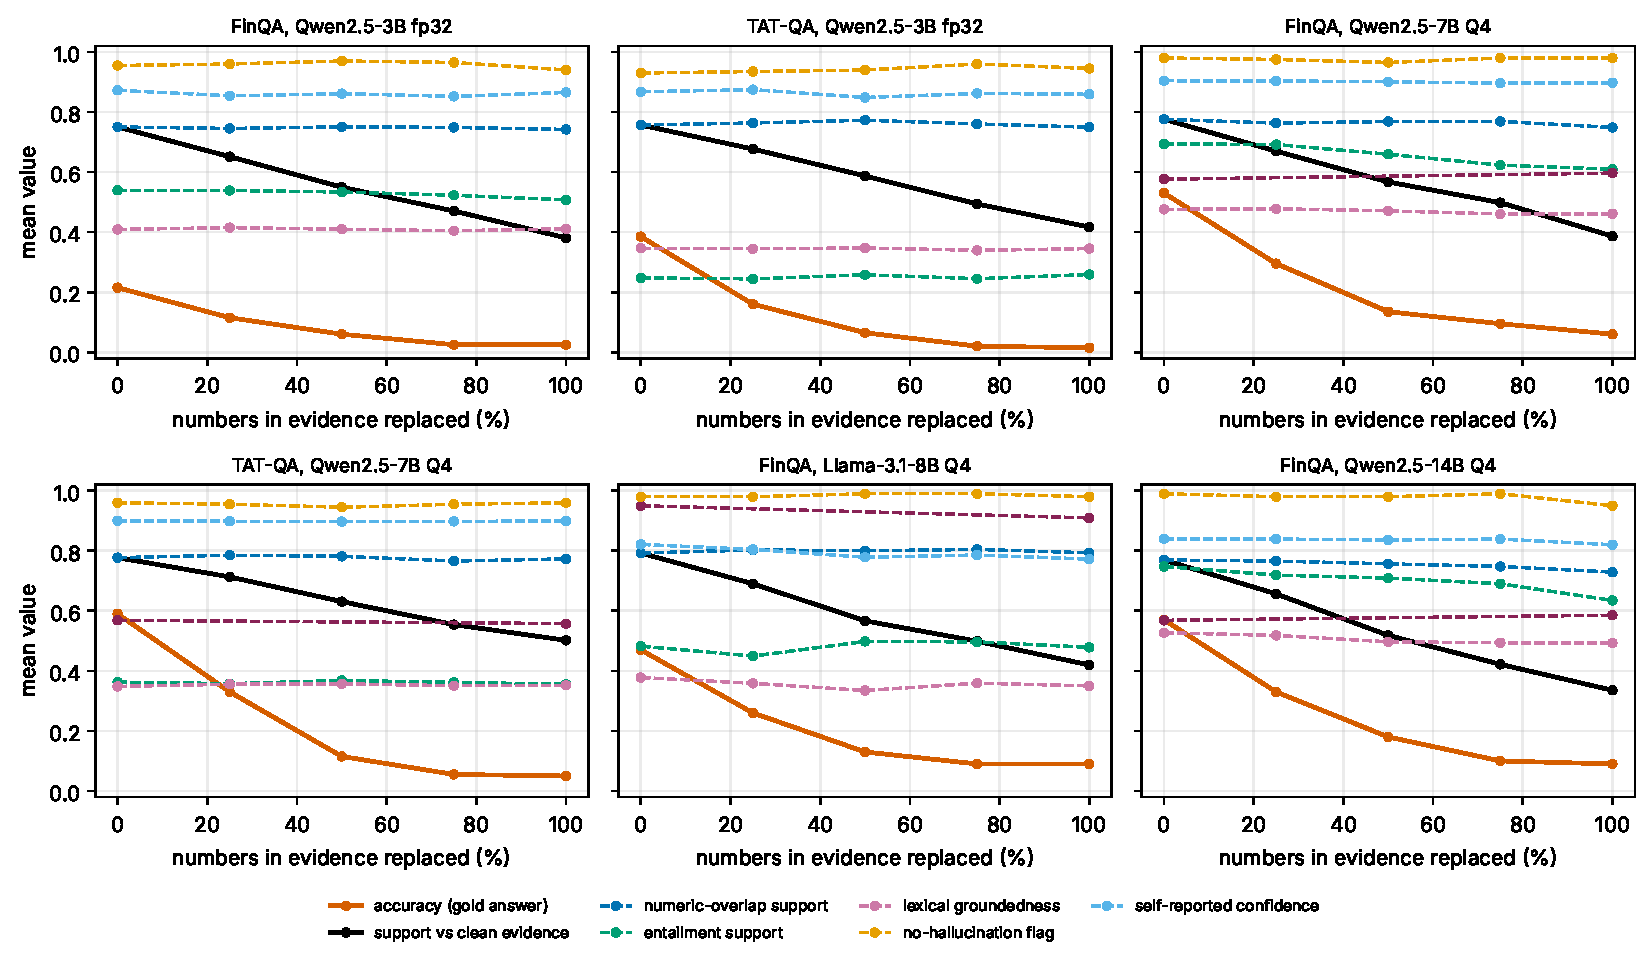
\includegraphics[width=\textwidth]{figures/corruption.pdf}
\caption{Mean value of each measure against the share of numbers in the retrieved evidence that were replaced by wrong ones (dev and test runs averaged within a dataset and model; 100 items per run). Solid lines need the gold answer or the clean evidence; dashed lines use only the response and the evidence shown to the model.}
\label{fig:corruption}
\end{figure}

Table~\ref{tab:paired} gives the paired change per item from $0\%$ to $100\%$ corruption.
Accuracy falls by 0.19 to 0.45 depending on run, and support against the clean evidence by 0.33 to 0.41.
The gold-free measures move by at most a few points.
For the 7B model, numeric-overlap and entailment support decline slightly but reliably (about $-0.03$ and $-0.09$), an order of magnitude less than accuracy.

\begin{table}[t]
\centering\small
\resizebox{\textwidth}{!}{\begin{tabular}{@{}l r ccccc@{}}
\toprule
Run & $n$ & accuracy$^\dagger$ & numeric-overlap support & entailment support & hallucination flag & support vs clean$^\ddagger$ \\
\midrule
FinQA / Qwen2.5-3B fp32 dev & 100 & -0.19 \small[-0.27, -0.12] & +0.00 \small[-0.02, +0.03] & +0.02 \small[-0.04, +0.07] & +0.01 \small[-0.04, +0.06] & -0.36 \small[-0.40, -0.33] \\
FinQA / Qwen2.5-3B fp32 test & 100 & -0.19 \small[-0.27, -0.11] & -0.02 \small[-0.06, +0.02] & -0.07 \small[-0.14, -0.00] & +0.02 \small[-0.03, +0.07] & -0.38 \small[-0.42, -0.33] \\
TAT-QA / Qwen2.5-3B fp32 dev & 100 & -0.37 \small[-0.46, -0.28] & +0.00 \small[-0.03, +0.03] & +0.04 \small[-0.02, +0.10] & -0.02 \small[-0.07, +0.03] & -0.35 \small[-0.39, -0.31] \\
TAT-QA / Qwen2.5-3B fp32 test & 100 & -0.37 \small[-0.46, -0.28] & -0.02 \small[-0.04, +0.01] & -0.02 \small[-0.08, +0.03] & -0.01 \small[-0.05, +0.02] & -0.33 \small[-0.36, -0.30] \\
FinQA / Qwen2.5-7B Q4 test & 100 & -0.45 \small[-0.55, -0.35] & -0.03 \small[-0.06, -0.01] & -0.09 \small[-0.16, -0.02] & +0.01 \small[-0.02, +0.05] & -0.41 \small[-0.44, -0.37] \\
TAT-QA / Qwen2.5-7B Q4 test & 100 & -0.58 \small[-0.68, -0.47] & -0.02 \small[-0.05, -0.00] & -0.03 \small[-0.09, +0.03] & +0.02 \small[-0.02, +0.06] & -0.29 \small[-0.33, -0.25] \\
FinQA / Llama-3.1-8B Q4 test & 100 & -0.38 \small[-0.48, -0.28] & +0.00 \small[-0.03, +0.03] & +0.00 \small[-0.07, +0.07] & +0.00 \small[-0.03, +0.03] & -0.37 \small[-0.41, -0.34] \\
\bottomrule
\end{tabular}}
\caption{Change from $0\%$ to $100\%$ corruption, paired within item, with 95\% bootstrap intervals over items. $^\dagger$ needs the gold answer. $^\ddagger$ needs the clean evidence.}
\label{tab:paired}
\end{table}

The question is whether a measure can \emph{tell} the two situations apart, not only whether its average moves.
Table~\ref{tab:corrupt-auroc} reports the AUROC for separating a response generated from fully corrupted evidence from one generated from the clean evidence of the same item.
Every gold-free measure is close to chance: pooled over runs, numeric-overlap support gives \aucFinoverlap{} \aucFinoverlapci{} on FinQA and \aucTatoverlap{} \aucTatoverlapci{} on TAT-QA, entailment support \aucFinnli{} and \aucTatnli{}, and the hallucination flag \aucFinnohalluc{} and \aucTatnohalluc{}.
Individual runs reach at most 0.58.
Accuracy, which needs the gold answer, reaches \aucFincorrect{} and \aucTatcorrect{} (it is limited because many clean responses are already wrong), and support against the clean evidence reaches \aucFinvsclean{} and \aucTatvsclean{}.
The information that distinguishes the two cases is in the pair (response, clean evidence), which a deployed system does not have.

\begin{figure}[t]
\centering
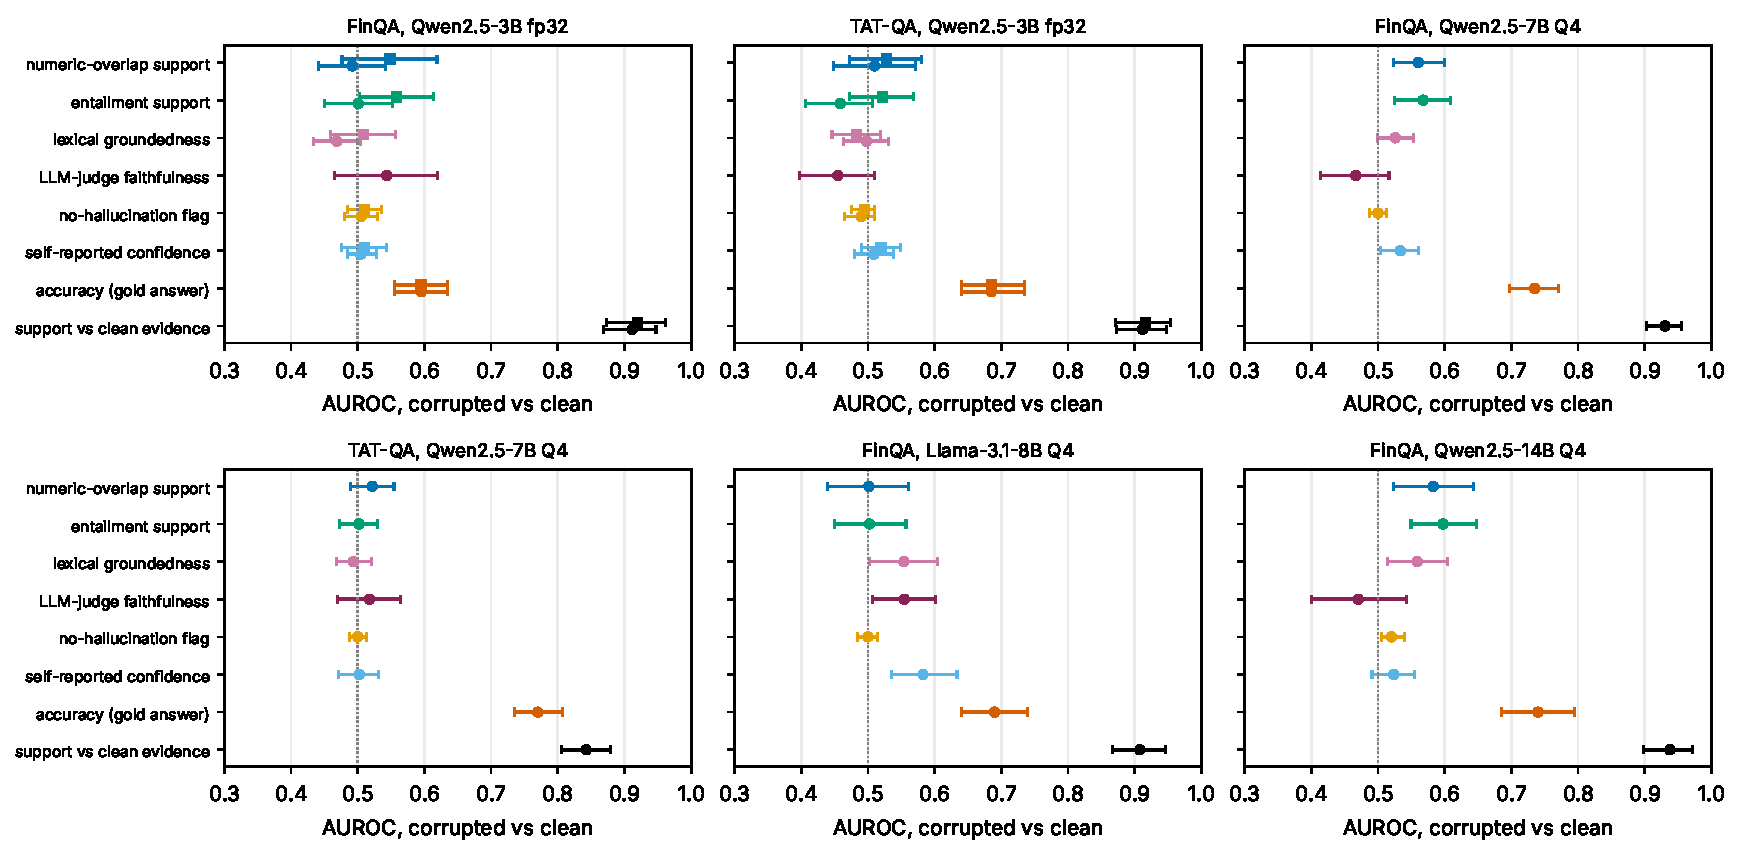
\includegraphics[width=\textwidth]{figures/auroc.pdf}
\caption{AUROC for telling a response produced from $100\%$-corrupted evidence from one produced from clean evidence (95\% bootstrap intervals over items; one marker per run). The dotted line is chance.}
\label{fig:auroc}
\end{figure}

\begin{table}[t]
\centering\small
\resizebox{\textwidth}{!}{\begin{tabular}{@{}l r ccccccc@{}}
\toprule
Run & $n$ & numeric-overlap support & entailment support & lexical groundedness & no-hallucination flag & self-reported confidence & accuracy$^\dagger$ & support vs clean$^\ddagger$ \\
\midrule
FinQA / Qwen2.5-3B fp32 dev & 100 & 0.49 \small[0.44, 0.54] & 0.50 \small[0.45, 0.55] & 0.47 \small[0.43, 0.50] & 0.51 \small[0.48, 0.53] & 0.50 \small[0.48, 0.52] & 0.59 \small[0.56, 0.64] & 0.91 \small[0.87, 0.95] \\
FinQA / Qwen2.5-3B fp32 test & 100 & 0.55 \small[0.48, 0.63] & 0.56 \small[0.51, 0.62] & 0.51 \small[0.46, 0.55] & 0.51 \small[0.49, 0.54] & 0.51 \small[0.48, 0.54] & 0.59 \small[0.55, 0.63] & 0.92 \small[0.87, 0.96] \\
\midrule
FinQA pooled & 200 & 0.52 \small[0.48, 0.57] & 0.53 \small[0.50, 0.57] & 0.49 \small[0.46, 0.51] & 0.51 \small[0.49, 0.53] & 0.51 \small[0.49, 0.53] & 0.59 \small[0.57, 0.62] & 0.92 \small[0.89, 0.94] \\
\bottomrule
\end{tabular}}
\caption{AUROC (95\% interval) for separating $100\%$-corrupted from clean evidence. $^\dagger$ needs the gold answer. $^\ddagger$ needs the clean evidence. Pooled rows combine the runs above them.}
\label{tab:corrupt-auroc}
\end{table}

The composite behaves accordingly.
Its correlation with the corruption level over the five levels is between $-0.90$ and $-0.97$ in every run, with intervals that exclude zero, and it comes entirely from the accuracy term and from the calibration term, which is a function of accuracy.
Replacing numeric-overlap support by support against the clean evidence in the composite changes little, because the composite is already dominated by accuracy.
So the composite does fall with corrupted evidence, but only through the terms that need the gold answer.

\subsection{Detecting wrong answers on clean evidence}

On clean evidence the gold-free measures should be useful if they carry information about errors.
Table~\ref{tab:error} shows they carry little.
Pooled over runs, AUROC for separating correct from incorrect answers is \errFinoverlap{} for numeric-overlap support, \errFinnli{} for entailment support, \errFinlexical{} for lexical groundedness, \errFinnohalluc{} for the hallucination flag and \errFinconf{} for verbalized confidence on FinQA (TAT-QA: \errTatoverlap, \errTatnli, \errTatlexical, \errTatnohalluc, \errTatconf).
Some individual runs deviate from 0.5 in both directions; for the 7B model numeric-overlap support is \emph{below} 0.5 on FinQA, because correct answers contain a computed result that is, by construction, not in the evidence, while a wrong answer that merely copies a figure scores as fully supported.
Verbalized confidence is nearly constant (most responses say 0.9), so its AUROC is uninformative regardless of model.
The lexical baseline performs no better than the entailment or overlap scores, so the weakness is not particular to the numeric-overlap design.

\begin{table}[t]
\centering\small
\resizebox{\textwidth}{!}{\begin{tabular}{@{}l r r ccccc@{}}
\toprule
Run & $n$ & Acc. & numeric-overlap support & entailment support & lexical groundedness & no-hallucination flag & self-reported confidence \\
\midrule
FinQA / Qwen2.5-3B fp32 dev & 100 & 0.22 & 0.60 \small[0.46, 0.73] & 0.49 \small[0.36, 0.62] & 0.52 \small[0.41, 0.65] & 0.53 \small[0.51, 0.56] & 0.53 \small[0.49, 0.59] \\
FinQA / Qwen2.5-3B fp32 test & 97 & 0.22 & 0.47 \small[0.32, 0.62] & 0.57 \small[0.43, 0.71] & 0.62 \small[0.48, 0.74] & 0.50 \small[0.44, 0.54] & 0.50 \small[0.47, 0.54] \\
FinQA / Qwen2.5-3B fp32 dev & 149 & 0.26 & 0.64 \small[0.55, 0.73] & 0.53 \small[0.43, 0.63] & 0.48 \small[0.38, 0.57] & 0.53 \small[0.51, 0.55] & 0.53 \small[0.49, 0.57] \\
FinQA / Qwen2.5-3B fp32 test & 145 & 0.21 & 0.52 \small[0.41, 0.64] & 0.55 \small[0.44, 0.67] & 0.57 \small[0.44, 0.69] & 0.51 \small[0.47, 0.54] & 0.53 \small[0.49, 0.58] \\
FinQA / Qwen2.5-1.5B fp32 dev & 100 & 0.40 & 0.44 \small[0.33, 0.54] & 0.51 \small[0.41, 0.61] & 0.46 \small[0.35, 0.59] & 0.52 \small[0.47, 0.56] & 0.53 \small[0.44, 0.61] \\
FinQA / Qwen2.5-1.5B fp32 test & 97 & 0.34 & 0.48 \small[0.36, 0.60] & 0.50 \small[0.39, 0.61] & 0.48 \small[0.35, 0.60] & 0.54 \small[0.51, 0.57] & 0.55 \small[0.45, 0.63] \\
FinQA / SmolLM2-1.7B fp32 dev & 100 & 0.16 & 0.32 \small[0.20, 0.47] & 0.42 \small[0.26, 0.61] & 0.36 \small[0.24, 0.52] & 0.47 \small[0.38, 0.54] & 0.50 \small[0.50, 0.50] \\
\midrule
FinQA pooled & 788 & 0.25 & 0.50 \small[0.46, 0.55] & 0.51 \small[0.47, 0.55] & 0.51 \small[0.47, 0.55] & 0.52 \small[0.50, 0.53] & 0.54 \small[0.52, 0.57] \\
\bottomrule
\end{tabular}}
\caption{AUROC for separating correct from incorrect answers under clean evidence (numeric questions only; 95\% bootstrap intervals over items).}
\label{tab:error}
\end{table}

\subsection{Real retrieval misses}

Corruption is synthetic.
A natural failure of the same kind occurs when the retriever does not surface the numbers the answer needs.
Table~\ref{tab:retrieval} compares items by whether the retrieved evidence contains every number of the gold evidence.
The miss rate is $\approx$\missFin\% on FinQA and varies by dataset definition on TAT-QA.
Accuracy is much lower on misses than on hits.
Whether a gold-free measure notices is inconsistent: pooled over FinQA runs numeric-overlap support gives AUROC \retFinoverlap{}, entailment \retFinnli{}, lexical groundedness \retFinlexical{}; for the 3B model on TAT-QA numeric-overlap support reaches 0.69, because with the needed figures absent the model invents or substitutes numbers that are then not in the evidence.
That is a different failure from corrupted evidence: \emph{missing} evidence can leave a trace in the response, whereas \emph{wrong} evidence leaves none.
Even where overlap support helps, accuracy itself separates hits from misses at least as well (FinQA pooled \retFincorrect).

\begin{table}[t]
\centering\small
\resizebox{\textwidth}{!}{\begin{tabular}{@{}l r r r cccccc@{}}
\toprule
Run & $n$ & Miss & Acc. hit / miss & numeric-overlap support & entailment support & lexical groundedness & no-hallucination flag & self-reported confidence & accuracy$^\dagger$ \\
\midrule
FinQA / Qwen2.5-3B fp32 dev & 150 & 0.13 & 0.29 / 0.00 & 0.53 \small[0.38, 0.68] & 0.60 \small[0.48, 0.70] & 0.48 \small[0.34, 0.61] & 0.53 \small[0.47, 0.60] & 0.61 \small[0.52, 0.72] & 0.65 \small[0.61, 0.69] \\
FinQA / Qwen2.5-3B fp32 test & 150 & 0.20 & 0.23 / 0.07 & 0.59 \small[0.47, 0.71] & 0.49 \small[0.38, 0.60] & 0.43 \small[0.29, 0.56] & 0.51 \small[0.47, 0.56] & 0.47 \small[0.38, 0.54] & 0.58 \small[0.52, 0.63] \\
FinQA / Qwen2.5-1.5B fp32 dev & 100 & 0.12 & 0.44 / 0.08 & 0.51 \small[0.32, 0.69] & 0.47 \small[0.30, 0.66] & 0.43 \small[0.23, 0.61] & 0.51 \small[0.45, 0.61] & 0.36 \small[0.22, 0.51] & 0.68 \small[0.56, 0.76] \\
FinQA / Qwen2.5-1.5B fp32 test & 100 & 0.17 & 0.39 / 0.06 & 0.57 \small[0.41, 0.73] & 0.58 \small[0.43, 0.73] & 0.48 \small[0.35, 0.64] & 0.54 \small[0.47, 0.63] & 0.44 \small[0.31, 0.56] & 0.66 \small[0.58, 0.73] \\
FinQA / SmolLM2-1.7B fp32 dev & 100 & 0.12 & 0.18 / 0.00 & 0.47 \small[0.30, 0.65] & 0.56 \small[0.43, 0.70] & 0.44 \small[0.26, 0.60] & 0.45 \small[0.42, 0.48] & 0.50 \small[0.50, 0.50] & 0.59 \small[0.56, 0.63] \\
\midrule
FinQA pooled & 600 & 0.15 & 0.30 / 0.04 & 0.54 \small[0.47, 0.61] & 0.53 \small[0.47, 0.59] & 0.45 \small[0.38, 0.52] & 0.51 \small[0.49, 0.54] & 0.48 \small[0.43, 0.52] & 0.63 \small[0.59, 0.65] \\
\bottomrule
\end{tabular}}
\caption{Items split by whether the retrieved evidence contains every number of the gold evidence (FinQA: annotated gold facts; TAT-QA: operands of the annotated derivation). AUROC: can the measure tell complete from incomplete retrieved evidence? $^\dagger$ needs the gold answer.}
\label{tab:retrieval}
\end{table}

\section{Correcting the earlier version}
\label{sec:erratum}

This study began as an evaluation of the ONRS composite on FinQA using 4-bit models on a consumer GPU.
Re-running it with more items and a test split exposed three problems, which we report because the earlier numbers are public.
\begin{enumerate}[leftmargin=*,itemsep=2pt,topsep=2pt]
\item \textbf{A scoring flaw.} The evidence-support score counted every number in the response, including the one in the model's own ``Confidence: 0.9'' line, which no evidence can support. Every response carried one extra unsupported number, lowering all support scores and pushing some under the hallucination threshold on that number alone. After removing the confidence statement, the hallucination rates reported earlier ($0.08$ in the baseline, $0.10\rightarrow0.20$ under noise) are $0.00$ in every condition.
\item \textbf{A manipulation that did not work.} The noise experiment added up to four sentences about unrelated figures. At 150 items per split the paired per-item change in accuracy between $0$ and $40\%$ noise was $+0.007$ (95\% interval $-0.05$ to $+0.07$) on dev and $-0.027$ ($-0.08$ to $+0.02$) on test. The injected text reached the model but did not hurt it, so a metric could not be faulted for failing to track it. Corrupting the numbers of the evidence (Section~\ref{sec:setup}) is the replacement.
\item \textbf{Unstable summary statistics.} The original conclusion that the composite fails to track noise and that no weighting of its four components rescues it came from a correlation over five noise-level means and a sweep of 1{,}771 weightings. On the same 3B model the correlation is $+0.09$ on dev and $-0.64$ on test, each with an interval of about $\pm0.8$, and the share of weightings passing both of the original falsification tests is $0.0\%$ on dev and $41.2\%$ on test. The results do not support a ranking of composites.
\end{enumerate}
A statement from the earlier version survives: evidence-support measures that compare a response with the supplied evidence cannot detect corrupted evidence.
It was an argument then; Section~\ref{sec:results} makes it an experiment.
The full list of corrected claims is in the repository (\texttt{ERRATUM.md}).

\section{Discussion}

\paragraph{What the results do and do not say.}
The tests do not show that overlap, entailment or judge scores are useless.
They measure faithfulness to the supplied context, and they do that job: a response that invents a number is flagged.
The finding is about what that property cannot cover.
When the failure is in the evidence, any score defined relative to the evidence reports ``faithful'' and is wrong about reliability.
A composite that adds such a score to accuracy and calibration moves with corruption only through the two terms that depend on the gold answer, and so is no better than accuracy at a task where accuracy is unavailable.

\paragraph{What gets past the limit.}
Only checks that bring in something outside the response and the evidence it was given.
The cheapest such signal, redundancy inside the evidence, is weak and fails when numbers are moved rather than changed.
A trusted copy of the numbers handles changed numbers but not moved ones, which is the more realistic failure of a mis-parsed table.
The check that handled every error we tried compares (row, column, value) cells with a trusted structured source, such as the XBRL record behind a filing. It needs that source to exist and the evidence to carry table structure, which limits it to part of the items (a third on FinQA).
Where such a source exists the practical conclusion is simple: verify the evidence against it before generation, and do not read a faithfulness score as a reliability estimate.

\paragraph{Implications for practice and for evaluation.}
(i) A reliability pipeline needs a signal about the evidence, not only about the response.
(ii) A verifier that compares numbers is not enough; compare structure.
(iii) Validate an evidence-quality manipulation by its effect on the model before using it to evaluate a metric. The distractor sentences we first used would have been reported as a metric failure.

\section{Conclusion}

Reference-free reliability scores for numerical RAG cannot see wrong evidence, and a controlled test on two datasets and four generators from two model families confirms it: accuracy collapses while every measure that sees only the response and the supplied evidence stays near chance (AUROC at most 0.60).
Realistic errors that merely misplace genuine numbers cost as much accuracy and escape even a check of the numbers against the clean evidence; only a cell-level check against a trusted structured copy catches them.
The same response-side measures are weak and model-dependent at flagging wrong answers on clean evidence and real retrieval misses.
Practitioners who need reliability estimates should treat such scores as faithfulness checks and add a verification of the evidence against a trusted structured source.

\section*{Limitations}

The generators are open models of 1.5B to 14B parameters, run without fine-tuning; larger or finance-tuned models may behave differently, and the 14B model was run on 100 items.
Accuracy is low for the smaller models (about 0.2 on FinQA for the 3B model; 0.47 to 0.62 for the 7B and larger models), which limits the power of the correct-versus-incorrect comparisons; we report intervals instead of claiming equality.
The scaled-number corruption is synthetic and numeric. The realistic errors (swapped periods and rows) are closer to real parsing failures but are still injected, were run for one generator (Qwen2.5-7B) and only on table rows, and on FinQA affect only the quarter to third of items whose retrieved evidence has an eligible table row.
The cell-level check is, by construction, an upper bound: it assumes a trusted structured copy and that the evidence carries table structure.
The retrieval-miss analysis defines a miss by the absence of gold numbers in the retrieved text, which can disagree with whether the answer was recoverable; the TAT-QA gold evidence is the operands of the annotated derivation because the dataset has no cell-level evidence labels.
The entailment measure uses one small NLI model; the lexical baseline is a heuristic; the faithfulness judge is a single 4-bit 8B model with one prompt, run only on the clean and fully edited evidence, and a stronger judge or a different prompt may do better. It is a RAGAs-\emph{style} score, not the RAGAs implementation.
The 7B, 8B and 14B models are 4-bit builds run through a different inference engine than the float32 models, so differences between sizes are confounded with precision.
We do not report a GPU 4-bit run of the smaller models.
Item counts (100 to 200 per run) are modest; pooling over runs narrows the intervals but mixes models.

\section*{Reproducibility}
Code, prompts, per-response outputs for every run, and the GitHub Actions workflow that regenerates them on free CPU runners are at \url{https://github.com/aaronsunny007/Financial-NRF}. Tables and figures in this paper are produced from the result files by \texttt{experiments/paper\_analysis.py} and \texttt{experiments/paper\_figures.py}.

\section*{Acknowledgements}
The experiments, analysis code and a first draft of this text were produced with the assistance of Claude (Anthropic), working in an agentic coding environment. The author directed the study, reviewed the results and the text, and is responsible for all claims. No external funding supported this work.


\bibliography{references}

\end{document}
